\documentclass{article}
\usepackage[utf8x]{inputenc}
\usepackage[pdftex]{graphicx}
\usepackage[mathletters]{ucs}
\usepackage{color}
\usepackage{ragged2e}
\setlength\parindent{3ex} 
\title{Relatório para a Atividade Acadêmica de Grafos}
\author{Ícaro.S.Barcelos Pereira, Michael Bruno Antunes da Silva,\\Matheus Willian Manhaes De Barros}
\date{Novembro 2019}

\begin{document}

\maketitle

\section{Resumo}

\hspace{\parindent}O relatório a seguir tem como objetivo exibir um algoritmo para o reconhecimento de grafos Hamiltonianos. Este problema é completo em NP, o que significa que é pouco provável que exista um algoritmo polinomial para o\\ problema. Portanto, serão apresentados um algoritmo de força bruta e uma versão otimizada do mesmo, que serão comparadas entre si.\par

\pagebreak
\section{Introdução}
\hspace{\parindent}Um grafo é dito hamiltoniano se possui um ciclo hamiltoniano, ou seja,\\ apresenta um ciclo que percorre todos os vértices do grafo. Uma das aplicações mais famosas dessa classe é no problema do caixeiro-viajante, que será abordado em breve.\par

\section{Propriedades de grafos hamiltonianos}
1 - Se G é um grafo hamiltoniano então para todo conjunto não-vazio \\S $\subset V (G), c(G - S) ≤ |S| $ (condição necessária para um grafo ser hamiltoniano).\\
\\2 - Se G é um grafo simples de ordem n ≥ 3 e g(v) ≥ n/2 para todo v ∈ V (G), então G é hamiltoniano (condição suficiente para um grafo ser \\hamiltoniano).\\

Prova 1. Suponha que a afirmação seja falsa. Então existe um grafo simples não-hamiltoniano
maximal G de ordem n ≥ 3 que satisfaz a condição do \\teorema. Ou seja, (maximal no sentido de que) G é não-hamiltoniano, mas para qualquer par de vértices não-adjacentes u, v em G, temos que o grafo G + uv é hamiltoniano.\par
Claramente G não é completo (todo grafo completo com pelo menos 3 vértices é obviamente hamiltoniano). Portanto, existem vértices u e v não-adjacentes em G. Considere o grafo H := G + uv. Pela maximalidade de G, segue que H é hamiltoniano. Logo, todo circuito hamiltoniano em H deve conter a aresta uv. Então G tem um caminho hamiltoniano, digamos\\
P := (u = v1, v2, . . . , vn = v).\\ Note que, se vi é adjacente a u, então vi−1 não é adjacente a v, pois senão\\ 
C = (v1, vi, vi+1, . . . , vn, vi−1, vi−2, . . . , v1)\\
seria um circuito hamiltoniano em G, contrariando a escolha de G.
Portanto, para todo vértice adjacente a u, existe um vértice de V (G) \ {v} que não é adjacente a v. Mas neste caso, g(v) ≤ n − 1 − g(u).\par
Como g(u) ≥ n/2, temos que g(v) ≤ n − 1 − n/2 = n/2 − 1, uma\\ contradição. Logo, a afirmação é verdadeira, e o teorema está provado.\\
\noindent
\\A prova em 2 motivou o seguinte resultado, cuja prova segue analogamente. Note que 2 é um corolário de 3.\\
\\3 - Se G é um grafo simples de ordem n ≥ 3 tal que
g(u) + g(v) ≥ n para todo par u, v de vértices não-adjacentes,
então G é hamiltoniano.\par
\pagebreak
\noindent
O seguinte resultado também foi motivado pela prova de 2. Note que a prova é análoga a que fizemos para 2.\\

4 - Seja G um grafo simples de ordem n e sejam u, v vértices não-adjacentes em G tais que g(u) + g(v) ≥ n. Então G é hamiltoniano se e só se G + uv é hamiltoniano.

\section{Problema do caixeiro-viajante}

\hspace{\parindent}O Problema do Caixeiro Viajante (PCV) é um problema que tenta\\ determinar a menor rota para percorrer uma série de cidades (visitando uma única vez cada uma delas), retornando à cidade de origem. É um problema de otimização NP-difícil inspirado na necessidade dos vendedores em realizar entregas em diversas cidades percorrendo o menor caminho possível, reduzindo o tempo necessário para a viagem e os possíveis custos com transporte e combustível.

\subsection{Definição}

\hspace{\parindent}O problema do caixeiro-viajante consiste na procura de um circuito que possua a menor distância, começando numa cidade qualquer, entre várias, visitando cada cidade precisamente uma vez e regressando à cidade inicial.\\
\\-Dado um conjunto {\displaystyle C=\{c_{1}\;,...,\;c_{n}\}}{\displaystyle C=\{c_{1}\;,...,\;c_{n}\}}$ de n cidades ci e uma matriz de distâncias {\displaystyle \left(\rho _{ij}\right)}{\displaystyle \left(\rho _{ij}\right)}, onde {\displaystyle \rho _{ij}=\rho (c_{i},\;c_{j})}{\displaystyle \rho _{ij}=\rho (c_{i},\;c_{j})} {\displaystyle (}( {\displaystyle i,\;j}{\displaystyle i,\;j} {\displaystyle \in }\in  {\displaystyle \{1,\;...,\;n\}}{\displaystyle \{1,\;...,\;n\}}, {\displaystyle \rho _{ij}}{\displaystyle \rho _{ij}} {\displaystyle =\rho _{ji}}{\displaystyle =\rho _{ji}}, {\displaystyle \rho _{ii}}{\displaystyle \rho _{ii}}{\displaystyle =0)}{\displaystyle =0)}$, a tarefa passa por\\ encontrar a permutação {\displaystyle \pi \in S_{n}=\{s:\{1,...,n\}\rightarrow \{1,...,n\}\}}{\displaystyle \pi \in S_{n}=\{s:\{1,...,n\}\rightarrow \{1,...,n\}\}}$ que faça com que a função objectivo (distância do circuito) {\displaystyle f:S_{n}\rightarrow \mathbb {R} }{\displaystyle f:S_{n}\rightarrow \mathbb {R} }$, onde

         
  
    
    {\displaystyle f(\pi )=\sum _{i=1}^{n-1}\rho \pi (i),\pi (i+1)+\rho \pi (n),\pi (1)}
  
{\displaystyle f(\pi )=\sum _{i=1}^{n-1}\rho \pi (i),\pi (i+1)+\rho \pi (n),\pi (1)}$,
atinja o seu mínimo.\\

O tamanho do espaço de procura aumenta exponencialmente dependendo de n, o número de cidades, uma vez que existem

    {\displaystyle (n-1)!/2\approx {1 \over 2}{\sqrt {2\pi (n-1)}}\left({\frac {n-1}{e}}\right)^{n-1}}
  
{\displaystyle (n-1)!/2\approx {1 \over 2}{\sqrt {2\pi (n-1)}}\left({\frac {n-1}{e}}\right)^{n-1}}$
\\circuitos possíveis (a posição inicial é arbitrária, e a ordem do circuito pode ser invertida).

\pagebreak

\subsection{Motivações}

\begin{itemize}
    \item A problemática do PCV pode ser entendida facilmente, uma vez que se aproxima dos problemas populares do mundo real;
    \item O PCV demonstra o caso mais simples dos problemas de requisição que são de enorme relevância para a programação de processos industriais;
    \item Existem vários conjuntos de dados sobre o PCV que estão disponíveis em literatura, de tal forma que os resultados são comparáveis mesmo que o ótimo global não seja ainda definitivamente conhecido;
    \item Relativamente à complexidade computacional, o PCV, como um problema NP-completo, é conhecido por representar uma larga classe de problemas para os quais não existem algoritmos polinomiais em séries temporais determinísticos.
\end{itemize}

\subsection{Formulação gráfica}

\hspace{\parindent}Cada cidade é identificada com um nó (ou vértice) e as rotas que ligam cada par de nós são identificadas como arcos (ou arestas). A cada uma destas linhas estarão associadas as distâncias (ou custos) correspondentes. Desde que seja possível ir diretamente de uma cidade para qualquer outra, o gráfico diz-se completo. Uma viagem que passe por todas as cidades corresponde a um ciclo Hamiltoniano, representado por um conjunto específico de linhas. A distância do ciclo é o somatório das distâncias das linhas presentes no mesmo.

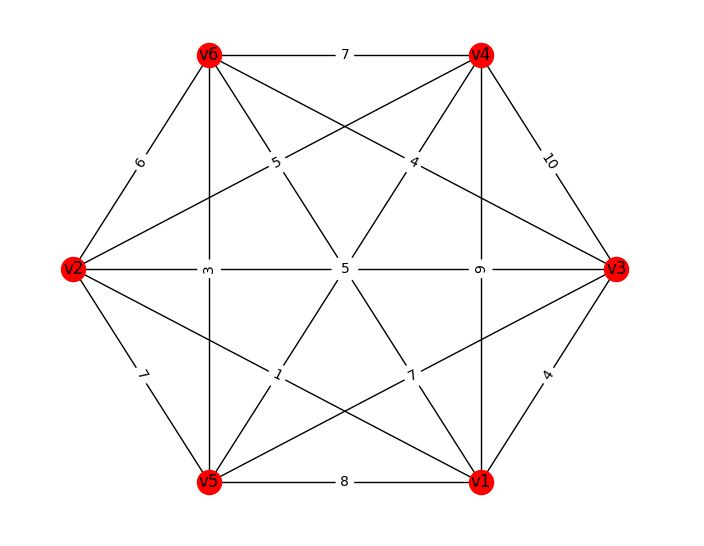
\includegraphics[scale=0.4]{Caixeiro.jpg}
\\exemplo de grafo hamiltoniano

\pagebreak

\section{Algoritmos}

\subsection{Grafo hamiltoniano}

função hamiltoniano\\
Entrada: vértice do grafo a ser analisado\\
Saída: grafo hamiltoniano, se existir\\

se (vértice vizinho == vértice inicial) retorne grafo; fim se\\

senão:

\hspace{\parindent}enquanto (número de vizinhos visitados $\ll$ número de vizinhos)\par\\
\hspace{6ex}escolhe vértice vizinho não visitado\par\\
\hspace{6ex}se(vizinho.visitado == falso)\par\\
\hspace{9ex}vizinho.visitado = verdadeiro\par
\hspace{9ex}hamiltoniano(analisa vizinho)\par
\hspace{6ex}fim se\par
\hspace{\parindent}fim enquanto\par\\
fim senão\\

retorne não\\
fim função

\subsection{Caixeiro-viajante}

função Caixeiro-viajante\\
Entrada: vértices do grafo indicando as cidades
\\Saída: melhor solução, caso exista\\

se (solução atual \gg$ melhor solução) retorne solução atual; fim se\\

senão:

\hspace{\parindent}enquanto (existir vértice para analisar)\par\\
\hspace{6ex}escolhe vértice da lista a ser analisado\par\\
\hspace{6ex}se(vértice.visitado == falso && custo \ll infinito)\par\\
\hspace{9ex}vértice.visitado = verdadeiro\par
\hspace{9ex}incrementa valor da solução atual\par
\hspace{9ex}Caixeiro-viajante(próximo vértice)\par
\hspace{6ex}fim se\par
\hspace{\parindent}fim enquanto\par\\
fim senão

fim função

\pagebreak

\section{Desempenho e instruções de uso}

Para compilar: gcc grafos.c -o grafos\\
Para executar: ./grafos\\

\subsection{Desempenho}
\begin{itemize}
    \item Tempo médio de execução (Caixeiro-viajante + identificação de grafo hamiltoniano num grafo de 6 vértices): 13.06 ms.
    \item Memória utilizada: 3072 bytes.
\end{itemize}

\subsection{Equipamento utilizado}
\begin{itemize}
    \item Intel Core i5-3230M com 2.6GHz de clock.
    \item 8 GB de memória RAM.
    \item Sistema operacional de 64 bits.
\end{itemize}

\section{Referências}

\begin{itemize}
    \item https://pt.wikipedia.org/wiki/Problema\_do\_caixeiro-viajante
    \item https://pt.wikipedia.org/wiki/Caminho\_hamiltoniano
    \item https://malbarbo.pro.br/arquivos/2013/6898/11-caminho-hamiltoniano-e-o-problema-do-caixeiro-viajante.pdf
    \item https://www.ime.usp.br/\tilde$ pf/algoritmos\_para\_grafos/aulas/max-weight-paths.html
    \item https://www.redalyc.org/jatsRepo/4675/467553545011/html/index.html
\end{itemize}
\end{document}